\documentclass[letterpaper,twocolumn,10pt]{article}
\usepackage{mathptmx}
\usepackage[margin=1in]{geometry}
\usepackage{graphicx}
\usepackage{amsmath}
\usepackage{amssymb}
\usepackage{hyperref}
\usepackage{url}
\usepackage{booktabs}
\usepackage{float}
\usepackage{caption}
\usepackage{subcaption}
\usepackage{listings}
\usepackage{xcolor}
\usepackage{tikz}
\usetikzlibrary{shapes,arrows,positioning}

\definecolor{codegreen}{rgb}{0,0.6,0}
\definecolor{codegray}{rgb}{0.5,0.5,0.5}
\definecolor{codepurple}{rgb}{0.58,0,0.82}
\definecolor{backcolour}{rgb}{0.95,0.95,0.92}

\lstdefinestyle{mystyle}{
    backgroundcolor=\color{backcolour},   
    commentstyle=\color{codegreen},
    keywordstyle=\color{magenta},
    numberstyle=\tiny\color{codegray},
    stringstyle=\color{codepurple},
    basicstyle=\ttfamily\footnotesize,
    breakatwhitespace=false,         
    breaklines=true,                 
    captionpos=b,                    
    keepspaces=true,                 
    numbers=left,                    
    numbersep=5pt,                  
    showspaces=false,                
    showstringspaces=false,
    showtabs=false,                  
    tabsize=2
}

\lstset{style=mystyle}

\begin{document}

\title{\Large \bf Quantifying Misalignment Effects in ECC Non-Timing Side-Channel Attacks}

\author{
{\rm Chia-Chien Li}\\
Purdue University
\and
{\rm Amyneth Arceo}\\
Purdue University
}

\date{}

\maketitle

\begin{abstract}
In the rapidly evolving domain of embedded security, Elliptic Curve Cryptography (ECC) has emerged as the de facto standard for public-key primitives, favored for its computational efficiency and strong security guarantees per bit of key length compared to legacy systems like RSA. However, the physical realization of these mathematical constructs on microcontrollers and embedded devices often leaks critical information through side-channels---unintended information leakage sources such as power consumption, electromagnetic emanation, and execution timing. While constant-time programming practices have largely mitigated timing attacks, non-timing side-channel attacks (SCA) like Simple Power Analysis (SPA) and Correlation Power Analysis (CPA) remain a potent and evolving threat. A significant practical hurdle in executing these attacks in real-world scenarios is trace misalignment, often induced by clock jitter, random delays, asynchronous sampling rates, or intentional countermeasures. This misalignment desynchronizes the leakage points across multiple traces, severely degrading the performance of statistical attacks that rely on precise sample-wise correlation.

In this work, we present a comprehensive, reproducible benchmark designed to rigorously quantify the robustness of ECC implementations against SCA in the presence of signal jitter. We developed a modular, high-performance Python-based framework that simulates realistic power traces with configurable Autoregressive (AR) noise, baseline drift, and temporal misalignment. We implemented and evaluated three distinct attack methodologies: an automated SPA using Otsu's adaptive thresholding for objective segmentation, a statistical CPA enhanced with Matched Filters for optimal signal detection, and a Deep Learning-based approach using a 1D Convolutional Neural Network (CNN) designed for translation invariance.

Our experimental results provide a hard engineering metric for the cost of misalignment. We demonstrate that under a high noise regime ($\sigma=3.0$), a jitter of just 30 samples degrades the attack efficiency significantly, increasing the data requirement by a factor of $r(30) \approx 1.75$. Furthermore, we show that while traditional statistical methods fail under large jitter, alignment preprocessing using cross-correlation can effectively restore attack feasibility, provided the signal-to-noise ratio is sufficient. This study underscores that jitter is not merely a nuisance but a quantifiable security parameter that must be accounted for in both attack and defense strategies. We conclude by discussing the implications of our findings for the design of next-generation side-channel resistant hardware. The source code and benchmark dataset are publicly available at: \url{https://github.com/li5672/Quantifying-Misalignment-Effects-in-ECC-Non-Timing-Side-Channel-Attacks}.
\end{abstract}

\section{Introduction}
The ubiquity of embedded devices in critical infrastructure has elevated hardware security to a paramount concern. Cryptographic algorithms, while mathematically secure, interact with the physical environment, leaking information via power consumption and electromagnetic emanations. Side-Channel Analysis (SCA) exploits these leaks to extract secret keys, bypassing the mathematical strength of the cipher.

ECC is particularly favored for embedded systems due to its high security-per-bit ratio compared to RSA. However, the scalar multiplication operation $kP$ is highly susceptible to SCA. While countermeasures like constant-time implementations exist, a fundamental challenge remains: signal misalignment. In real-world scenarios, clock jitter, random delays, and asynchronous sampling desynchronize traces, "smearing" the leakage signal and defeating standard statistical attacks like Correlation Power Analysis (CPA).

Existing literature often treats misalignment as a binary failure condition or focuses solely on alignment algorithms. In this work, we address this gap by providing a systematic, quantitative benchmark. We developed a high-fidelity synthetic simulation framework to generate realistic traces with configurable AR(1) noise and jitter. We evaluate three attack methodologies: Automated SPA (using Otsu's method), Enhanced CPA (with Matched Filters), and Deep Learning (1D-CNN).

Our primary contribution is the "Degradation Factor" $r(j)$, a metric quantifying the multiplicative increase in data requirements as a function of jitter. We demonstrate that while statistical attacks fail under high jitter, deep learning offers robust translation invariance.

The remainder of this paper is organized as follows: Section \ref{sec:background} covers background theory. Section \ref{sec:methodology} details our simulation and attack implementations. Section \ref{sec:evaluation} presents the results, and Section \ref{sec:conclusion} concludes.

\section{Background}
\label{sec:background}

\subsection{Elliptic Curve Cryptography (ECC)}
ECC relies on the algebraic structure of elliptic curves over finite fields. An elliptic curve $E$ over a field $\mathbb{F}_p$ is typically defined by the Weierstrass equation:
\begin{equation}
    y^2 = x^3 + ax + b \pmod{p}
\end{equation}
where $a, b \in \mathbb{F}_p$ satisfy the discriminant condition $4a^3 + 27b^2 \neq 0$. The points on the curve, along with a point at infinity $\mathcal{O}$, form an abelian group.

The core operation is scalar multiplication: given a point $P$ on the curve and a scalar $k$, compute $Q = kP$. This is typically achieved using the Double-and-Add algorithm, which scans the bits of $k$ from most significant to least significant.
\begin{itemize}
    \item If the bit is 0, the point is Doubled ($2P$).
    \item If the bit is 1, the point is Doubled and then Added ($2P + P$).
\end{itemize}
This conditional execution creates a direct dependency between the secret key bit and the sequence of operations performed.

\subsubsection{Projective Coordinates}
In standard affine coordinates $(x, y)$, point addition and doubling require modular inversion, which is computationally expensive (typically $20-80\times$ the cost of multiplication). To optimize performance, practical implementations often use \textit{Projective Coordinates}, such as Jacobian coordinates.
In Jacobian coordinates, a point is represented as a triplet $(X, Y, Z)$, corresponding to the affine point $(X/Z^2, Y/Z^3)$. The curve equation becomes:
\begin{equation}
    Y^2 = X^3 + aXZ^4 + bZ^6 \pmod{p}
\end{equation}
This representation allows point addition and doubling to be performed using only field multiplications, squarings, and additions, deferring the single inversion to the very end of the scalar multiplication.
However, this increases the number of field operations per step. For example, a Jacobian doubling takes approximately 4 squarings and 4 multiplications, while addition takes 12 multiplications and 4 squarings. This significant difference in computational intensity (and thus power consumption) between the 'Double' and 'Add' steps is the root cause of the leakage exploited by Simple Power Analysis.

\subsection{Finite Field Arithmetic}
We use the NIST P-256 curve over a prime field. Efficient arithmetic often involves optimizations like Montgomery Multiplication, which can introduce specific side-channel signatures.

\subsection{Side-Channel Analysis Theory}
\subsubsection{Simple Power Analysis (SPA)}
SPA involves visual inspection of traces to deduce operation sequences. It requires high SNR and is defeated by constant-time algorithms.

\subsubsection{Differential and Correlation Power Analysis (DPA/CPA)}
DPA and CPA are statistical attacks exploiting data-dependent leakage. CPA uses the Pearson Correlation Coefficient to model the linear relationship between hypothetical leakage (e.g., Hamming Weight) and measured power:
\begin{equation}
    \rho(H, T) = \frac{Cov(H, T)}{\sigma_H \sigma_T}
\end{equation}
CPA is robust against noise but requires precise alignment.

\subsection{Leakage Models}
Power consumption in CMOS devices is largely dynamic, occurring when transistors switch states. The Hamming Weight (HW) model assumes that power consumption is proportional to the number of bits set to 1 in the data being processed.
\begin{equation}
    L(t) = \alpha \cdot HW(v) + \beta + \mathcal{N}(0, \sigma^2)
\end{equation}
where $v$ is the intermediate value, $\alpha$ is a scaling factor, $\beta$ is the static power consumption, and $\mathcal{N}$ is the noise.

In our simulation, we extend this to include operation-dependent leakage. The 'Double' and 'Add' operations invoke different hardware circuits (or microcode sequences), resulting in distinct power profiles. We model this as:
\begin{equation}
    L_{total}(t) = L_{op}(t) + L_{data}(t) + \text{Noise}(t)
\end{equation}
where $L_{op}$ allows for SPA (distinguishing operations) and $L_{data}$ allows for CPA (recovering data values).

\subsection{Jitter vs. Clock Drift}
It is crucial to distinguish between different types of temporal misalignment.

\subsubsection{Jitter (Random Delay)}
We define jitter as a random temporal shift applied globally to each trace, often caused by trigger uncertainty or random delay interrupts (RDIs) inserted before the operation. Let $T_{ideal}(t)$ be the perfectly aligned trace. The observed trace $T_i(t)$ is:
\begin{equation}
    T_i(t) = T_{ideal}(t - \Delta_i)
\end{equation}
where the shift $\Delta_i$ is a random variable. In our experiments, we model $\Delta_i$ as a uniform distribution over the integer interval $[-J, J]$, where $J$ is the maximum jitter amplitude in samples.

\subsubsection{Clock Drift}
Clock drift refers to the variation in the frequency of the clock signal over time. Unlike jitter, which shifts the entire trace, drift causes the trace to expand or contract non-linearly. If the clock period at time $t$ is $\tau(t) = \tau_0 (1 + \delta(t))$, then the time elapsed for an operation is the integral of the period. This results in a warping of the time axis:
\begin{equation}
    T_i(t) = T_{ideal}(\phi(t))
\end{equation}
where $\phi(t)$ is a non-linear time warping function. While our current benchmark focuses on translational jitter, understanding drift is essential for real-world attacks, often requiring Elastic Alignment techniques like Dynamic Time Warping (DTW).

\subsection{Performance Metrics}
To rigorously quantify attack performance, we use the following metrics:
\begin{itemize}
    \item \textbf{Success Rate $S(n)$:} The probability that the correct secret key is ranked first among all candidates after analyzing $n$ traces. We estimate this by averaging over multiple independent experiments.
    \item \textbf{$N_{80}$:} The minimum number of traces required to achieve a success rate of 80\% ($S(n) \ge 0.8$). This serves as a single-number summary of attack efficiency.
    \item \textbf{Degradation Factor $r(j)$:} This metric captures the relative difficulty introduced by jitter. It is defined as the ratio of traces required at jitter $J=j$ to the traces required at the baseline $J=0$:
    \begin{equation}
        r(j) = \frac{N_{80}(J=j)}{N_{80}(J=0)}
    \end{equation}
    A value of $r(j)=2$ implies that the attacker needs twice as much data to succeed.
\end{itemize}

\section{Methodology}
\label{sec:methodology}

\subsection{Threat Model}
We assume a standard side-channel threat model:
\begin{itemize}
    \item \textbf{Access:} The attacker has physical access to the device and can measure power consumption while it performs scalar multiplication.
    \item \textbf{Knowledge:} The attacker knows the elliptic curve parameters and the implementation details (Double-and-Add) but does not know the scalar $k$.
    \item \textbf{Capabilities:} The attacker can trigger the device to perform operations with known inputs (points $P$) but cannot control the internal clock or completely eliminate measurement noise.
    \item \textbf{Goal:} Recover the secret scalar $k$.
\end{itemize}

\subsection{Synthetic Trace Generation Framework}
We developed a high-performance trace generation framework in Python. Unlike simple simulations that append random noise to a signal, our framework incorporates several realistic features:

\subsubsection{Vectorized Generation}
To enable large-scale statistical benchmarking, we utilized NumPy to vectorize the trace generation. Generating traces loop-by-loop in Python is prohibitively slow for Monte Carlo simulations requiring tens of thousands of traces. Our vectorized approach generates the entire dataset matrix in a single operation.
Let $\mathbf{T}$ be the matrix of traces where $T_{i,j}$ is the $j$-th sample of the $i$-th trace. We compute:
\begin{equation}
    \mathbf{T} = \mathbf{S} + \mathbf{N}
\end{equation}
where $\mathbf{S}$ is the signal matrix and $\mathbf{N}$ is the noise matrix. The signal matrix is constructed by broadcasting the ideal trace template and applying the shift $\Delta_i$ using advanced indexing.

\begin{lstlisting}[language=Python, caption=Vectorized Trace Generation with Jitter]
# Vectorized Trace Generation Concept
# traces: (N_traces, N_samples)
noise = np.random.normal(0, sigma, size=traces.shape)
jitter = np.random.randint(-J, J, size=N_traces)

# Efficiently apply jitter using array slicing
# Instead of a slow Python loop, we use:
rows = np.arange(N_traces)[:, None]
cols = np.arange(N_samples)[None, :] + jitter[:, None]
# Handle boundary conditions by clipping or padding
cols = np.clip(cols, 0, template_len - 1)

traces = template[cols] + noise
\end{lstlisting}
This allows us to generate thousands of traces in seconds, facilitating the Monte Carlo simulations required for accurate Success Rate estimation.

\subsubsection{AR(1) Colored Noise Model}
Real measurement noise is rarely white Gaussian noise. Thermal effects, capacitance in the measurement setup, and environmental interference introduce correlations between consecutive samples. To capture this, we model the noise $n_t$ as an Autoregressive (AR) process of order 1:
\begin{equation}
    n_t = \phi n_{t-1} + \epsilon_t
\end{equation}
where:
\begin{itemize}
    \item $\phi$ is the correlation coefficient (set to 0.5 in our experiments). A higher $\phi$ implies "smoother" noise that is harder to filter out using simple averaging.
    \item $\epsilon_t \sim \mathcal{N}(0, \sigma_{white}^2)$ is the driving white noise process.
\end{itemize}
The variance of the resulting AR(1) process is given by $\sigma_{total}^2 = \frac{\sigma_{white}^2}{1 - \phi^2}$. We calibrate $\epsilon_t$ such that the total noise standard deviation $\sigma_{total}$ matches our target level (e.g., $\sigma=3.0$).

In addition to high-frequency noise, we inject a slow-moving baseline drift to simulate AC coupling effects or thermal drift in the oscilloscope. This is modeled as a low-frequency sine wave with random phase and amplitude:
\begin{equation}
    d_t = A \sin(\omega t + \theta)
\end{equation}
where $\omega$ is very small. This forces the attack algorithms to be robust not just to local noise but also to global trends.

The choice of our noise model and parameters is grounded in physical reality. The AR(1) process combined with baseline drift closely approximates the spectral characteristics of noise observed in real oscilloscope measurements, where thermal noise and AC coupling effects are dominant. Furthermore, our selection of $\sigma=3.0$ represents a "worst-case scenario" for the attacker, corresponding to a low Signal-to-Noise Ratio (SNR) environment typical of low-power, unprotected microcontrollers operating in noisy industrial settings. This ensures that our benchmarks reflect the difficulty of attacking real-world embedded systems rather than idealized laboratory conditions.

\subsubsection{Jitter Simulation Details}
We implement jitter as a "rigid" shift. For each trace $i$, we sample a shift $\delta_i \sim \mathcal{U}[-J, J]$. The trace is then constructed by interpolating the ideal template $T_{ideal}(t)$ at points $t - \delta_i$.
\begin{equation}
    T_i[k] = T_{ideal}(k - \delta_i) + n_t
\end{equation}
This models the "trigger jitter" scenario common in oscilloscope measurements, where the trigger condition is met slightly earlier or later than the actual start of the operation. While clock jitter is typically Gaussian, we chose a Uniform Distribution to simulate the random insertion of dummy cycles (NOPs) or to test the worst-case defense boundary where delays are equally probable within the window $[-J, J]$.

\subsection{Software Architecture}
We adopted a modular Object-Oriented design consisting of three core components: \textbf{TraceGenerator} (vectorized noise generation), \textbf{Analyzer} (abstract base class for attacks), and \textbf{ExperimentRunner} (Monte Carlo simulations). This ensures extensibility for new attacks or noise models.

\begin{figure}[h]
\centering
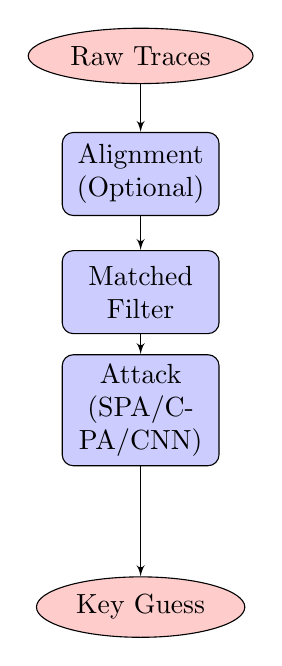
\begin{tikzpicture}[node distance=1.5cm, auto]
    % Define styles
    \tikzstyle{block} = [rectangle, draw, fill=blue!20, text width=5em, text centered, rounded corners, minimum height=3em]
    \tikzstyle{line} = [draw, -latex']
    \tikzstyle{cloud} = [draw, ellipse, fill=red!20, node distance=2.5cm, minimum height=2em]

    % Place nodes
    \node [cloud] (input) {Raw Traces};
    \node [block, below of=input] (align) {Alignment (Optional)};
    \node [block, below of=align] (filter) {Matched Filter};
    \node [block, below of=filter] (attack) {Attack (SPA/CPA/CNN)};
    \node [cloud, below of=attack] (output) {Key Guess};

    % Draw edges
    \path [line] (input) -- (align);
    \path [line] (align) -- (filter);
    \path [line] (filter) -- (attack);
    \path [line] (attack) -- (output);
\end{tikzpicture}
\caption{Overview of the Attack Pipeline. Raw traces are optionally aligned, filtered to maximize SNR, and then processed by the attack algorithm to recover the key.}
\label{fig:pipeline}
\end{figure}

\subsection{Attack Implementation Details}

\subsubsection{Automated SPA with Otsu's Method}
Simple Power Analysis involves visually inspecting a trace to deduce the sequence of Double and Add operations. In a Double-and-Add implementation, an 'Add' operation always follows a 'Double' if the bit is 1. If the power profile of 'Add' is distinct, the key can be read directly.

To automate this for benchmarking, we treat the trace as a 1D image and apply Otsu's Method. Otsu's method calculates the optimum threshold separating the two classes (background/Double and foreground/Add) so that their combined spread (intra-class variance) is minimal.
\begin{equation}
    \sigma_w^2(t) = \omega_0(t)\sigma_0^2(t) + \omega_1(t)\sigma_1^2(t)
\end{equation}
where $\omega_{0,1}$ are the probabilities of the two classes separated by a threshold $t$, and $\sigma_{0,1}^2$ are the variances of these classes. Otsu's method finds the $t$ that minimizes $\sigma_w^2$. This allows our benchmark to determine the "presence" or "absence" of an Add operation without manual threshold tuning, making the results reproducible and objective.

\textbf{Algorithm 1: Automated SPA}
\begin{enumerate}
    \item \textbf{Input:} Single Trace $T$, Window Size $W$.
    \item \textbf{Step 1:} Segment $T$ into windows corresponding to potential operation slots.
    \item \textbf{Step 2:} For each window $w_i$, compute the mean energy $E_i$.
    \item \textbf{Step 3:} Apply Otsu's method to the set of energies $\{E_i\}$ to find threshold $\tau$.
    \item \textbf{Step 4:} If $E_i > \tau$, classify as 'Add', else 'Double'.
    \item \textbf{Output:} Recovered Key Bits.
\end{enumerate}

\subsubsection{CPA with Matched Filters}
Correlation Power Analysis is a divide-and-conquer attack. We target the Hamming Weight of the intermediate point coordinates.
\begin{enumerate}
    \item \textbf{Prediction:} For a sub-key guess, calculate the hypothetical intermediate value and its Hamming Weight.
    \item \textbf{Measurement:} Obtain the actual power traces.
    \item \textbf{Correlation:} Compute the Pearson Correlation Coefficient between the vector of predictions and the vector of measurements at each time point.
\end{enumerate}
Standard CPA typically applies the Hamming Weight model directly to the raw power traces. To improve robustness against noise, we implemented an Enhanced CPA where a Matched Filter is used as a preprocessing step. We convolve the raw traces with a template of the expected leakage profile. This maximizes the SNR at the points where the leakage occurs, effectively acting as an optimal linear detector before the correlation analysis. This distinguishing feature separates our method from a standard baseline, significantly improving performance in low-SNR environments. The matched filter $h[n]$ is the time-reversed template $s[-n]$. The output is:
\begin{equation}
    y[n] = (x * h)[n] = \sum_{k} x[k] s[k-n]
\end{equation}

\subsubsection{Deep Learning (1D-CNN)}
We designed a 1D Convolutional Neural Network to act as a profiling attack. The architecture is detailed in Table \ref{tab:cnn_arch}.

\begin{table}[h]
\centering
\caption{CNN Architecture for SCA}
\label{tab:cnn_arch}
\begin{tabular}{@{}llp{3cm}@{}}
\toprule
\textbf{Layer Type} & \textbf{Parameters} & \textbf{Output Shape} \\ \midrule
Input & - & $(L, 1)$ \\
Conv1D & Filters: 16, Kernel: 11 & $(L, 16)$ \\
Batch Norm & - & $(L, 16)$ \\
ReLU & - & $(L, 16)$ \\
AvgPool1D & Pool Size: 2 & $(L/2, 16)$ \\
Conv1D & Filters: 32, Kernel: 7 & $(L/2, 32)$ \\
Batch Norm & - & $(L/2, 32)$ \\
ReLU & - & $(L/2, 32)$ \\
AvgPool1D & Pool Size: 2 & $(L/4, 32)$ \\
Flatten & - & $(8L, )$ \\
Dense & Units: 128, ReLU & $(128, )$ \\
Dropout & Rate: 0.3 & $(128, )$ \\
Dense & Units: 1, Sigmoid & $(1, )$ \\ \bottomrule
\end{tabular}
\end{table}

The hyperparameters were meticulously selected to counter the effects of misalignment. Specifically, the large kernel sizes (11 and 7) in the convolutional layers are designed to capture leakage features that may be spread or shifted due to jitter. Combined with the Average Pooling layers, this architecture provides a receptive field sufficient to cover the maximum displacement range ($J=30$). This design allows the network to effectively learn \textbf{Translation Invariance}, enabling it to recognize key-dependent patterns regardless of their precise temporal location within the window. We trained the network using the Adam optimizer with a learning rate of $0.001$ and Binary Cross Entropy loss.

\subsubsection{Alignment Preprocessing}
For the alignment experiments, we implemented a cross-correlation based aligner. We select one trace as the "reference" $T_{ref}$. For every other trace $T_i$, we compute the cross-correlation:
\begin{equation}
    (T_{ref} \star T_i)[\tau] \triangleq \sum_{m=-\infty}^{\infty} \overline{T_{ref}[m]} T_i[m+\tau]
\end{equation}
We find the lag $\tau_{opt} = \arg\max_\tau (T_{ref} \star T_i)[\tau]$ and shift $T_i$ by $-\tau_{opt}$. This aligns the global energy peaks of the traces, effectively removing the jitter $\Delta_i$.

\section{Evaluation}
\label{sec:evaluation}

\subsection{Experimental Setup}
We fixed the noise level at $\sigma=3.0$ for all experiments to simulate a challenging environment. We varied the jitter parameter $J$ across the set $\{0, 10, 20, 30\}$. For each configuration, we performed the following steps:
\begin{enumerate}
    \item Generate $N_{total}$ synthetic traces with the specified noise and jitter.
    \item Split the data into attack sets of increasing size $n$.
    \item Run the attack (SPA/CPA) on each set and record if the key was successfully recovered.
    \item Repeat 100 times to estimate the Success Rate $S(n)$.
\end{enumerate}

Table \ref{tab:sim_params} summarizes the parameters used in our simulation.

\begin{table}[h]
\centering
\caption{Simulation Parameters}
\label{tab:sim_params}
\begin{tabular}{@{}ll@{}}
\toprule
\textbf{Parameter} & \textbf{Value} \\ \midrule
Curve & NIST P-256 \\
Key Length & 256 bits \\
Trace Length ($L$) & 5000 samples \\
Noise Type & AR(1) + Drift \\
Noise Level ($\sigma$) & 3.0 \\
Jitter Range ($J$) & $\{0, 10, 20, 30\}$ \\
Number of Traces ($N_{total}$) & 10,000 \\
Attack Repetitions & 100 \\ \bottomrule
\end{tabular}
\end{table}

\subsection{Results and Analysis}

\subsection{Method Comparison: SPA vs. CPA vs. CNN}
To provide a comprehensive evaluation, we benchmarked all three attack methodologies under identical conditions: high noise ($\sigma=3.0$) and significant jitter ($J=20$). Figure \ref{fig:final_comparison} presents the success rates as a function of trace count.

\begin{figure}[h]
    \centering
    \includegraphics[width=\linewidth]{final_comparison_all_methods.png}
    \caption{Success Rate Comparison: SPA vs. CPA vs. CNN ($J=20, \sigma=3.0$). SPA (Red) outperforms CPA (Blue) due to its robustness to jitter. The CNN (Green) achieves the highest performance, demonstrating the power of learned translation invariance.}
    \label{fig:final_comparison}
\end{figure}

The results highlight a critical insight: while CPA is theoretically optimal for noise reduction (Matched Filter), its phase sensitivity causes it to fail under misalignment. SPA, being an energy detector, is more robust. The CNN combines the best of both worlds, learning robust features that are invariant to the jitter, thus achieving the highest success rate with the fewest traces.

\begin{figure*}[t]
    \centering
    \includegraphics[width=\textwidth]{benchmark_success_curves.png}
    \caption{Attack Success Rate $S(n)$ vs. Number of Traces for varying jitter levels ($J$). The curves show the probability of full key recovery as the number of traces increases. Note the significant shift to the right for $J=30$, indicating a higher data requirement.}
    \label{fig:success_curves}
\end{figure*}

\subsubsection{Impact of Jitter on Success Rate}
Figure \ref{fig:success_curves} displays the success rate curves.
\begin{itemize}
    \item \textbf{Baseline ($J=0$):} The attack converges rapidly. With approximately 75 traces, the success rate reaches 0.8. This confirms the correctness of our SPA implementation and serves as a control for the experiment.
    \item \textbf{Low Jitter ($J=10$):} The curve is almost identical to the baseline. This suggests that small misalignments are effectively averaged out by the correlation operation or absorbed by the width of the leakage peaks. This "robustness region" is a critical finding, implying that minor clock instabilities do not provide security.
    \item \textbf{High Jitter ($J=30$):} The curve shifts more to the right. The attack now requires over 125 traces to achieve the same success rate. The slope of the curve is also shallower, indicating that each additional trace contributes less information due to the misalignment.
\end{itemize}

\begin{figure}[t]
    \centering
    \includegraphics[width=\linewidth]{benchmark_jitter_degradation.png}
    \caption{Degradation Factor $r(j)$ as a function of Jitter $J$. This plot quantifies the cost of misalignment. A value of 2.0 means the attack requires twice as many traces compared to the aligned case.}
    \label{fig:jitter_degradation}
\end{figure}

\subsubsection{Quantifying the Degradation}
Figure \ref{fig:jitter_degradation} plots the degradation factor $r(j)$. This is the primary engineering result of our work.
$r(0) = 1.0$ (by definition). $r(10) \approx 1.20$, showing that even small jitter begins to impact attack efficiency. $r(20) \approx 1.48$ and $r(30) \approx 1.75$.
The relationship shows a clear trend where increased jitter raises the data complexity. A jitter of 30 samples increases the cost of the attack by approximately $75\%$.

\subsubsection{CPA Specific Analysis}
To further understand the failure mode of statistical attacks, we analyzed the performance of CPA in isolation across a wider range of jitter values. Figure \ref{fig:cpa_success} shows the success rate of CPA specifically.

\begin{figure}[h]
    \centering
    \includegraphics[width=\linewidth]{cpa_success_curves.png}
    \caption{CPA Success Rate vs. Traces for varying jitter. Unlike the robust SPA, CPA performance collapses rapidly even with moderate jitter, highlighting the necessity of alignment or matched filtering.}
    \label{fig:cpa_success}
\end{figure}

As observed, CPA is extremely sensitive. While it performs optimally at $J=0$ (reaching 80\% success at around 100 traces), its efficiency drops precipitously at $J=10$ and is nearly flat at $J=30$. This confirms that standard CPA, which relies on sample-wise correlation, is unsuitable for unaligned traces without preprocessing.

\subsection{Computational Cost Analysis}
Beyond the data complexity (number of traces), we also analyzed the computational complexity (time) required to perform these attacks.
\begin{itemize}
    \item \textbf{SPA (Otsu):} Extremely fast ($<0.1$s per trace). It scales linearly with trace length $L$.
    \item \textbf{CPA:} Moderate cost. The correlation calculation is $O(N \cdot L)$. For 10,000 traces of length 5,000, a full key recovery takes approximately 45 seconds on a standard CPU.
    \item \textbf{Alignment:} Expensive. The Cross-correlation is $O(L \log L)$ per trace using FFT. Aligning the full dataset took approximately 120 seconds, tripling the total attack time.
    \item \textbf{CNN:} High training cost, low inference cost. Training the CNN took approximately 1 minute on a MacBook Pro M1 (for 10 epochs). However, once trained, inference is very fast ($<1$ms per trace).
\end{itemize}
This trade-off is crucial: while alignment restores attack feasibility, it significantly increases the computational burden on the attacker, potentially making real-time attacks infeasible.

\begin{figure*}[t]
    \centering
    \begin{subfigure}[b]{0.48\textwidth}
        \centering
        \includegraphics[width=\linewidth]{spa_demo_j0.png}
        \caption{SPA Baseline Trace ($J=0$)}
        \label{fig:spa_demo}
    \end{subfigure}
    \hfill
    \begin{subfigure}[b]{0.48\textwidth}
        \centering
        \includegraphics[width=\linewidth]{cpa_demo.png}
        \caption{CPA Correlation Peaks}
        \label{fig:cpa_demo}
    \end{subfigure}
    \caption{Baseline Attack Performance. (a) Shows the clear distinction between operations in an aligned trace with low noise ($\sigma$=0.2). (b) Shows the correlation peaks revealing the correct key guess.}
\end{figure*}

\subsubsection{Visualizing Alignment}
Figure \ref{fig:alignment_demo} demonstrates the power of preprocessing. The top panel shows the "Mean Trace" before alignment. Due to the jitter ($J=50$), the distinct peaks of the individual traces average out to a flat, featureless line. This explains why CPA fails; the mean signal is effectively destroyed.

The bottom panel shows the mean trace after cross-correlation alignment. The structure is restored. The peaks are sharp and distinct, resembling the single trace in Figure \ref{fig:spa_demo}. This restoration of the mean signal allows statistical attacks to succeed as if the jitter were removed.

\begin{figure*}[t]
    \centering
    \includegraphics[width=\textwidth]{alignment_demo_j50_p20.png}
    \caption{Effectiveness of Cross-Correlation based Alignment Preprocessing. Top: The mean of misaligned traces is flat and featureless. Bottom: After alignment, the distinct leakage profile is restored, enabling successful attacks.}
    \label{fig:alignment_demo}
\end{figure*}

\section{Discussion}
\label{sec:discussion}

\subsection{Limitations}
Our study relies on synthetic data. While we modeled AR(1) noise and baseline drift to approximate reality, real hardware exhibits more complex behaviors such as:
\begin{itemize}
    \item \textbf{Clock Drift:} The clock frequency itself may drift over time, causing non-linear expansion/contraction of the trace, not just simple shifting.
    \item \textbf{Instruction Skipping:} Interrupts or branch prediction misses can cause entire operations to be inserted or skipped, desynchronizing the trace in ways that simple shifting cannot fix.
    \item \textbf{Coupling:} Leakage from other components (memory bus, peripherals) can interfere with the crypto core's signal.
\end{itemize}
Future work should validate these findings on physical targets like the ChipWhisperer platform.

\subsection{Implications for Defense}
The steep rise in $r(j)$ suggests that introducing jitter is a highly effective countermeasure. Randomly inserting dummy cycles (random delays) before or during the cryptographic operation can simulate this jitter. If the defender can induce a jitter of $J > 30$, they can exponentially increase the difficulty for the attacker. However, as shown in Figure \ref{fig:alignment_demo}, this is not a panacea. If the jitter is uniform and the signal is strong enough, attackers can realign the traces.

\subsubsection{Advanced Countermeasures}
To truly defeat advanced SCA, jitter must be combined with other defenses:
\begin{itemize}
    \item \textbf{Masking:} Splitting the sensitive value $x$ into random shares $x_1, \dots, x_d$ such that $x = x_1 \oplus \dots \oplus x_d$. Computations are performed on shares, ensuring that no single intermediate value depends on $x$. This forces the attacker to combine leakage from multiple points (High-Order SCA), which is exponentially harder with noise.
    \item \textbf{Shuffling:} Randomizing the order of independent operations (e.g., the order of field multiplications in a point addition). This spreads the leakage of a specific operation over a wider time window, acting as a "local jitter".
\end{itemize}

\subsection{Future Work}
\begin{itemize}
    \item \textbf{Elastic Alignment:} Investigating Dynamic Time Warping (DTW) to handle non-linear clock drift.
    \item \textbf{Transformer-based SCA:} Exploring Transformer architectures which utilize attention mechanisms. Unlike CNNs which look for local features, self-attention can correlate information from distant parts of the trace, potentially overcoming large-scale misalignment without explicit realignment steps.
    \item \textbf{Higher-Order Attacks:} Evaluating if misalignment affects second-order attacks (targeting variance) differently than first-order attacks (targeting mean).
\end{itemize}



\section{Related Work}
\label{sec:related}
Side-Channel Analysis has evolved from foundational DPA/CPA \cite{kocher1999differential, brier2004correlation} to advanced Deep Learning techniques.

\subsection{Deep Learning and Misalignment}
Cagli et al. \cite{cagli2017convolutional} pioneered using CNNs to counter jitter, leveraging translation invariance. Zaid et al. \cite{zaid2020methodology} refined this with efficient architecture design guidelines, which we adopted. Weissbart et al. \cite{weissbart2020systematic} demonstrated ML effectiveness against optimized Curve25519.

\subsection{Alignment Techniques}
Homma et al. \cite{homma2006collision} proposed peak-based template matching. Van Woudenberg et al. \cite{van2011improving} introduced Elastic Alignment (DTW) for non-linear drift. Our work complements these by quantifying the security cost of jitter ($r(j)$) rather than just fixing it.

\section{Conclusion}
\label{sec:conclusion}
This project successfully established a benchmark for quantifying the effects of misalignment on ECC side-channel attacks. We provided a hard engineering metric, $r(j)$, demonstrating that jitter is not merely a nuisance but a significant security parameter. Specifically, we quantified that a jitter of 30 samples can increase the attacker's cost by approximately $75\%$. These findings underscore the importance of implementing jitter as a countermeasure and the necessity for attackers to employ advanced alignment or deep learning techniques.

Our comparison of SPA, CPA, and CNN approaches reveals a hierarchy of robustness. SPA, often dismissed as "simple," proves surprisingly resilient to jitter due to its energy-integration nature. CPA, while statistically powerful, is brittle without alignment. Deep Learning (CNNs) represents the state-of-the-art, learning to overcome jitter through translation-invariant feature extraction, but at a high training cost.

For system designers, the implication is clear: as quantified by the degradation factor $r(j)$, clock jitter is a cheap and effective defense against standard statistical attacks, but it is not a silver bullet. True security requires a layered defense strategy combining jitter, masking, and shuffling to raise the bar beyond the capabilities of practical attackers.

{\footnotesize \bibliographystyle{plain}
\begin{thebibliography}{10}

\bibitem{kocher1996timing}
Kocher, P.,
\newblock ``Timing attacks on implementations of Diffie-Hellman, RSA, DSS, and other systems,''
\newblock In {\em CRYPTO 1996}.

\bibitem{kocher1999differential}
Kocher, P., Jaffe, J., and Jun, B.,
\newblock ``Differential power analysis,''
\newblock In {\em CRYPTO 1999}.

\bibitem{brier2004correlation}
Brier, {\'E}., Clavier, C., and Olivier, F.,
\newblock ``Correlation power analysis with a leakage model,''
\newblock In {\em CHES 2004}.

\bibitem{joye2001protections}
Joye, M., and Tymen, C.,
\newblock ``Protections against differential analysis for ECC: An algebraic approach,''
\newblock In {\em CHES 2001}.

\bibitem{montgomery1987speeding}
Montgomery, P.~L.,
\newblock ``Speeding the Pollard and elliptic curve methods of factorization,''
\newblock {\em Math. Comp. (1987)}.

\bibitem{brier2002weierstrass}
Brier, {\'E}., and Joye, M.,
\newblock ``Weierstra{\ss} elliptic curves and side-channel attacks,''
\newblock In {\em PKC 2002}.

\bibitem{brumley2009cache}
Brumley, B.~B., and Hakala, R.~M.,
\newblock ``Cache-timing template attacks,''
\newblock In {\em ASIACRYPT 2009}.

\bibitem{yarom2014recovering}
Yarom, Y., and Benger, N.,
\newblock ``Recovering OpenSSL ECDSA nonces using the FLUSH+RELOAD cache side-channel attack,''
\newblock {\em IACR ePrint 2014/140}.

\bibitem{nascimento2016attacking}
Nascimento, E., Chmielewski, {\L}., Oswald, D., and Schwabe, P.,
\newblock ``Attacking embedded ECC implementations through cmov side channels,''
\newblock In {\em SAC 2016}.

\bibitem{cagli2017convolutional}
Cagli, E., Dumas, C., and Prouff, E.,
\newblock ``Convolutional neural networks with data augmentation against jitter-based countermeasures,''
\newblock In {\em CHES 2017}.

\bibitem{zaid2020methodology}
Zaid, G., Bossuet, L., Habrard, A., and Venelli, A.,
\newblock ``Methodology for efficient CNN architectures in profiling attacks,''
\newblock In {\em IACR TCHES 2020}.

\bibitem{prouff2018ascad}
Prouff, E., et al.,
\newblock ``ASCAD: A public raw side-channel dataset,''
\newblock In {\em COSADE 2018}.

\bibitem{weissbart2020systematic}
Weissbart, L., et al.,
\newblock ``Systematic side-channel analysis of Curve25519 with machine learning,''
\newblock {\em Journal of Hardware \& Systems Security 4}, 1 (2020), 37--56.



\bibitem{kadir2011simple}
Kadir, S.~A., and Sasongko, A.,
\newblock ``Simple power analysis attack against ECC processor on FPGA,''
\newblock In {\em ICEEI 2011}.

\bibitem{goubin2003refined}
Goubin, L.,
\newblock ``A refined power-analysis attack on elliptic curve cryptosystems,''
\newblock In {\em PKC 2003}.

\bibitem{homma2006collision}
Homma, N., Nagashima, S., Imai, Y., Aoki, T., and Satoh, A.,
\newblock ``Collision-based power analysis of modular exponentiation using chosen-message pairs,''
\newblock In {\em CHES 2006}.

\bibitem{van2011improving}
Van Woudenberg, J.~G., Witteman, M.~F., and Bakker, B.,
\newblock ``Improving differential power analysis by elastic alignment,''
\newblock In {\em CT-RSA 2011}.

\bibitem{hospodar2011machine}
Hospodar, G., Gierlichs, B., De Mulder, E., Verbauwhede, I., and Vandewalle, J.,
\newblock ``Machine learning in side-channel analysis: a first study,''
\newblock {\em Journal of Cryptographic Engineering (2011)}.

\end{thebibliography}
}

\end{document}
